\documentclass[10pt,a4paper]{article}
\usepackage[margin=1.2in]{geometry}
\usepackage{graphicx}
\usepackage{csquotes}
\usepackage{rotating}
\usepackage{amsmath}
\usepackage{algorithm}
\usepackage{mathtools}
\usepackage[noend]{algpseudocode}
\usepackage[justification=centering]{caption}
\renewcommand*{\refname}{Bibliography}


\begin{document}

\begin{titlepage}
    \begin{center}
        \vspace{1cm}
        
        \Huge
        \textbf{Visualising Ant Colonoy Optimisation}
        
	 \vspace{0.5cm}
       
        \huge
        \textbf{Design} \\
        
        \vspace{1.0cm}
        
        \Large
	 \textbf{Version:} 1.0 Draft \\
        G400  Computer Science, CS39440
	  

        \vspace{1.0cm}
        
	  \Large
        \textbf{Author:} Christopher Edwards \\
         che16@aber.ac.uk

 	  \vspace{0.8cm}
 	  \textbf{Supervisor:} Dr. Neil Mac Parthaláin \\
         ncm@aber.ac.uk
        
        \vspace{3.0cm}
        
        An overview of design and design rationale for a Computer Science Major Project
                
        \vspace{0.8cm}
                
        \Large
        Department of Computer Science\\
        Aberystwyth University\\
        Wales\\
        \today
        
	\end{center}
\end{titlepage}

\section{Language}

The choice of implementation language for both the graphical user interface and the Ant Colony Optimisation algorithm is extremely important. The nature of the project suggests that an Object Orientated approach would best suit as the implementation language. One of the main reasons for this is because the manipulation and use of Objects in such languages allows for Object-based decomposition allowing for more logical modules system wide when compared to a non-Object Orientated approach. A non-Object Orientated approach may be more subject to functional decomposition (the application is split into modules grouping similar functions rather than representing separate Objects).

An Object Orientated approach has been identified as most suitable. Therefore there are two main languages which are at the forefront of the selection process. These two languages are C\# (\textit{C Sharp}) and Java. Both languages have the potential to achieve a high level of success when applied to the project’s problem however; they both have different consequences depending on the environment and application in which they are used. C++ (\textit{C plus plus}) is another popular Object-Orientated language.  C++ has been discounted due to lack of language experience therefore using a more familiar language such as the two specified above (Java and C\#) is far more appropriate in this instance. 

One of the major factors in deciding on the implementation language is the suitability of the language’s features when applied to the projects problem including any external resources or compatible libraries. Both Java and C\# are very similar at an abstract level in terms of provided features by default. Both include everything that would be necessary to implement the proposed design for this application. Both languages provide the ability for Objective decomposition and allow for polymorphic behaviours (multiple entities of different types using the same interface) which enables effective use of inheritance to allow multiple Agent variations (Ants in this case) to be supported easily. 

C\# has been created and is continually being developed by Microsoft and is focused around the .NET framework which is also a product of Microsoft. As C\# is heavily Microsoft orientated its cross-platform capabilities are significantly reduced. The .NET framework(s) have only recently been open sourced so they lack full support on all platforms reducing the applications cross-platform reliability. The project is being developed with a focus on educational value; therefore cross-platform reliability is very important as maximisation of potential consumers is important (more people using the application implies more people are learning). A standard build will not be specified or assumed so there must be necessary measures in place to accommodate as many environments as possible. C\# is heavily coupled with Windows based systems therefore; If C\# were to be used there is a risk of alienating Macintosh and UNIX users. There are attempts to port .NET to other architectures (for example, Mono\cite{mono}) but the implementations of such approaches are not exact replicas of Microsoft .NET framework(s), therefore they cannot be relied upon. The use of Java would eliminate the cross-platform support issues as Java applications execute inside the Java Runtime Environment (JRE) which is available across most platforms and behaviours can be accurately modelled and predicted in the vast majority of cases.

Little differs between Java and C\# in terms of feature presence (abstractly, how each language achieves each task is very different) thus, Java will be used for this project. The cross-platform constraints that come with the use of C\# are not balanced by any necessary exclusive key features. As a result Java is the most appropriate language for the project, this all but ensures cross-platform reliability without sacrificing any important libraries or features.


\section{Architecure}

There have been considerations as to what key elements will be present in the composure of a suitable underlying architecture for the application. The architecture must accommodate both major elements of the application (graphical user interface and the Ant Colony Optimisation algorithm) in a manner that enables the best possible expansion/modification opportunities to accommodate any additional features or unforeseen changes. Selecting relevant Design Patterns will enable the above goals to become reality however; design patterns should be respectfully and must represent a general solution to a problem. The Overuse or misuse of such patterns can cause significant complexity issues through the system, this needs to be avoided. 

\subsection{Design and Architectural Patterns}

\subsubsection{Model-View-Controller}
\label{sssec:mvc}
\label{sec:patternsmvc}
The Model-View-Controller (MVC) Architectural Pattern is designed to reduced coupling between system components, these are represented here as the user interface(s) (View) and the underlying data and its representation(s) (Model). The interaction(s) between the View and the Model \enquote{established using a subscribe and notify protocol}\cite{gof:design:mvc} (Controller). The Controller updates the View(s) based on the model(s) current state or vice-versa however; The View(s) cannot directly communicate with the Model, the Controller must govern such interactions.

This project will make effective use of Model-View-Controller in order to produce an environment which is much easier to maintain and has little coupling between the Model and the View(s). This allows the Model(s) and/or View(s) to be substituted or modified in order allowing different representations of the current algorithm, or in fact different algorithms altogether. 

\begin{figure}[h]
\centering
\includegraphics[width=0.6\textwidth]{MVC}
\caption{Basic abstract overview of the Model-View-Controller pattern}
\end{figure}

\begin{itemize}
\item \textbf{Model} represents the underlying Ant Colony Optimisation algorithm. The Model also contains the required arithmetic functions and any additional operations required to execute the algorithm correctly.
\item \textbf{View} represents the graphical user interface which will not only display the algorithms execution, but also enable the user(s) to modify the algorithms parameters.
\item \textbf{Controller} represents the Observer required to enable interactions between the Model(s) and View(s).
\end{itemize}
\noindent

\subsubsection{Singleton}
\label{sssec:singleton}
In order to maintain simplicity throughout the application the Singleton design pattern will implemented for key Objects where one and only one instance of an Object must exist. The Singleton pattern prevents multiple instantiations of specific Object(s) as the Object itself is solely responsible for tracking the currently instantiated instance of itself\cite{gof:design:singleton}. 

The application will consist of a graphical user interface which in turn, will be composed of several different components. Such components must only be instantiated once in order to ensure correct interactions are performed. Without the presence of the Singleton pattern there exists the possibility of multiple instances of such components which could potentially cause unforeseen complications and undefined behaviours.

\begin{figure}[h]
\centering
\label{fig:singleton}
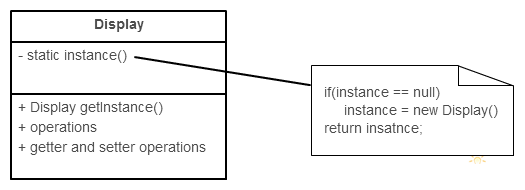
\includegraphics[width=0.8\textwidth]{signleton}
\caption{Proposed high-level implementation of the Singleton pattern demonstrating how the sole instance of the graphical user interface will be tracked.}
\end{figure}

\subsection{Structure}

Adhering to the concepts of the patterns described in sections \ref{sssec:mvc} and \ref{sssec:singleton} the following Class Diagram shows proposed application structure. This is not concrete and could potentially change throughout development, the Class Diagram in question is represented below by figure \ref{fig:classdiagram} and is represented using standard UML notation.

\clearpage
\begin{sidewaysfigure}
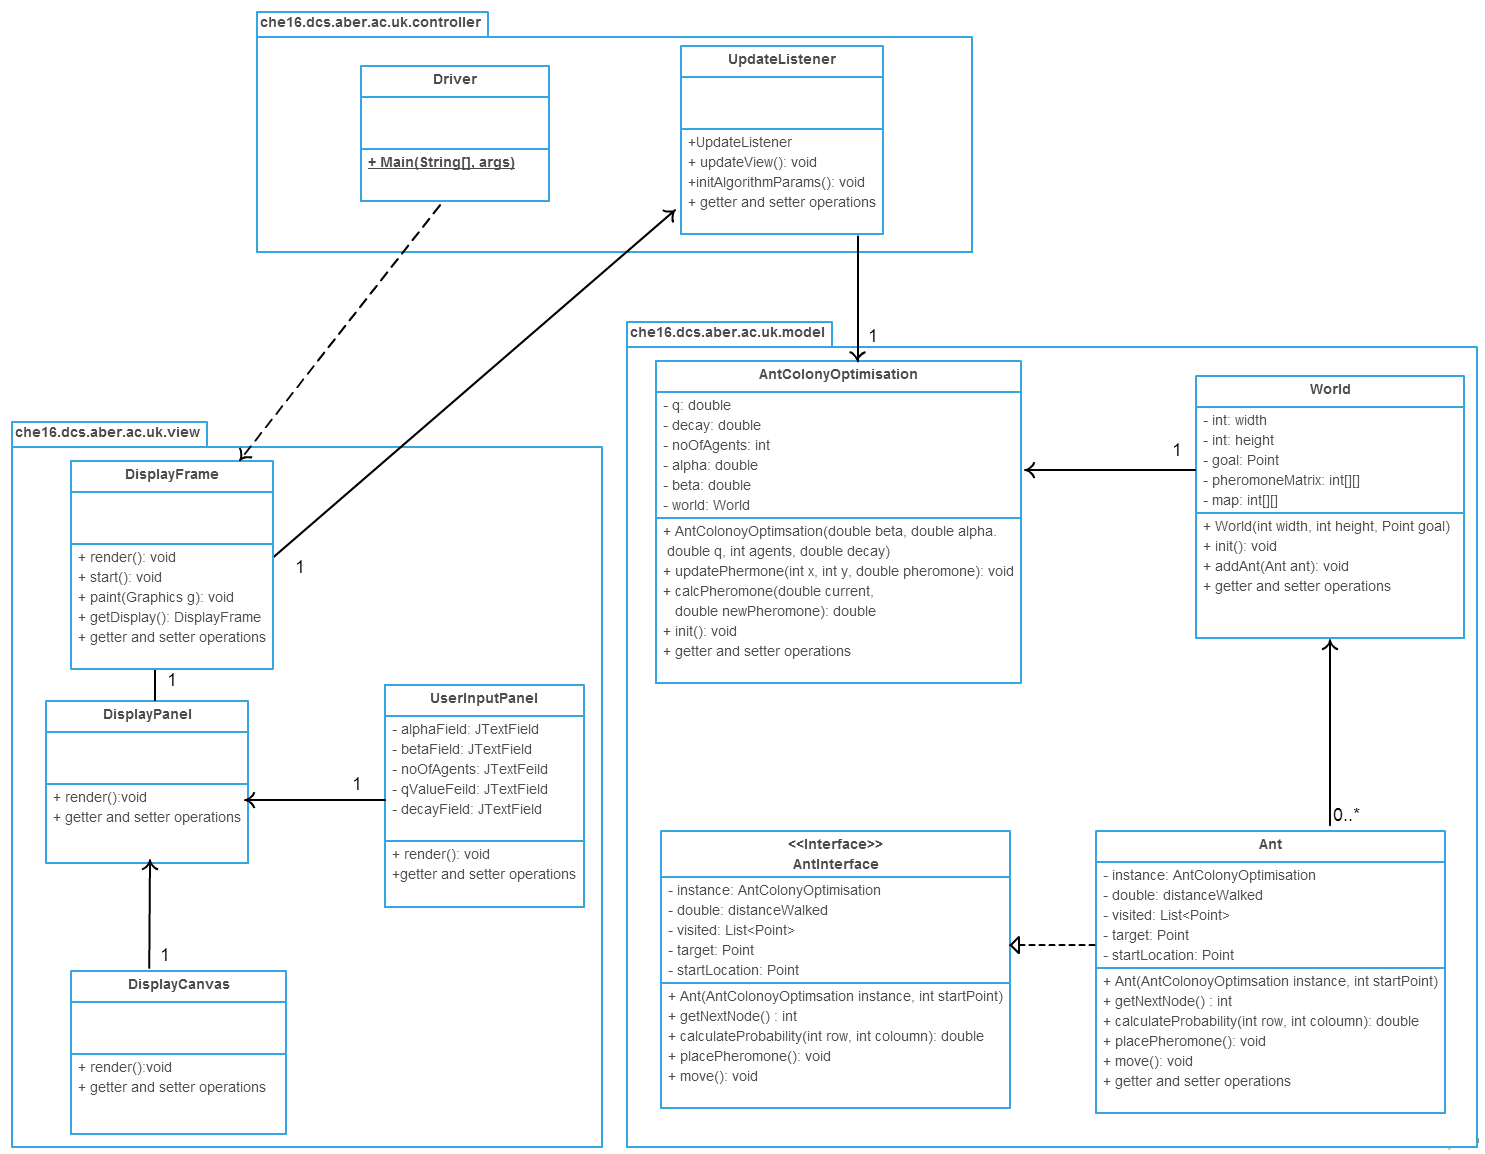
\includegraphics[scale=0.45]{raw-class-diagram}
\caption{Initial Class Diagram representing the main modules, packages and system interactions using UML notation.}
\label{fig:classdiagram}
\end{sidewaysfigure}
\clearpage

\subsubsection{View Package}

\label{sssec:view}
The $che16.dcs.aber.ac.uk.view$ package contains the graphical user interface components. The main concept behind this is the use of nested components such as JPanel, JTextFields and the like. These will be contained inside top level JFrame. This allows modification of each component in isolation without impacting the other components behaviours and/or elements. This is the first module of the application which is initialised, and is done so directly from the $main$ method. This package has no direct knowledge of any package members mentioned in \ref{sssec:model}. Instead the $che16.dcs.aber.ac.uk.controller$ package members handle the communication(s) between the model(s) and view(s), adhering to the principles discussed in section \ref{sssec:mvc}.

\subsubsection{Model Package}
\label{sssec:model}
The che16.dcs.aber.ac.uk.model package contains the necessary elements and attributes required in order to accurately represent the algorithms state(s) and ensure correct algorithm execution. This package has no directl knowledge of any package members mentioned in \ref{sssec:view}. Instead the controller package members handle the communication(s) between these the model(s) and view(s), adhering to the principles discussed in section \ref{sssec:mvc}.

\subsubsection{Controller Package}
The initial concept for the controller is basic and will grow in complexity during the development lifecycle as more and more control based mechanisms will become prevalent. This initial concept is a simple Observer which notifies the view(s) should the model change in a significant way; the inverse of this is also true.

\section{Interface Design}

The interface design must accommodate all the necessary elements required to allow user defined values for each of the algorithm parameters. The interface must also be able to visually represent the current algorithms state including the locations of the agents and nodes without impacting on the usability of the application (the interface must not freeze or be negatively affected by the algorithms execution).

The interface will use a very neutral colour scheme which will maximise the usability and reduce the risk of complications which may arise from users being subject to difficulties understanding or identifying certain colours. Every option for the user will be textually defined and will not rely on any sound or visual prompts in order to user. As a result in addition to the above, users with visual impairments will still be able to use the application as intended.

\begin{figure}[H]
\centering
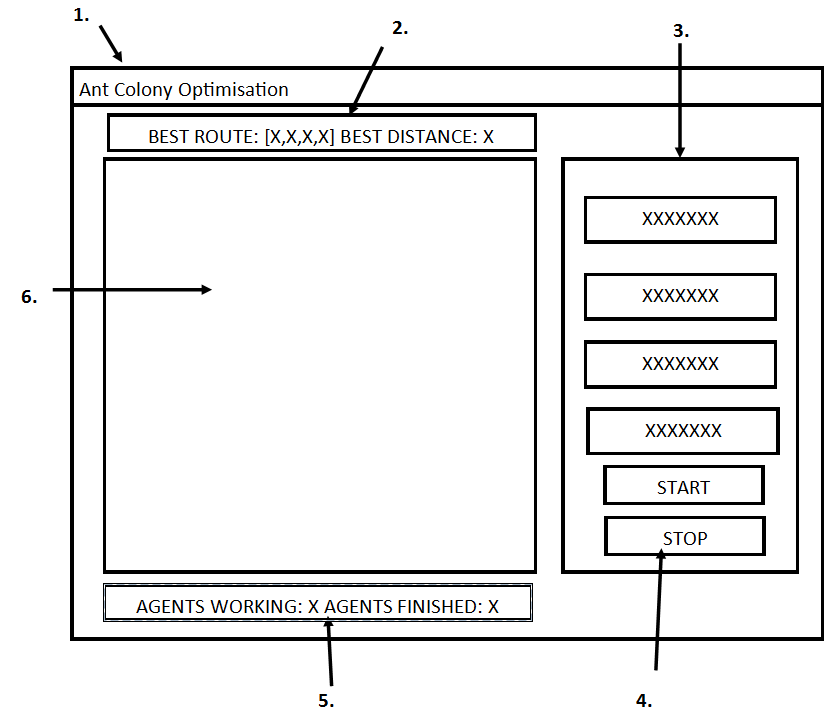
\includegraphics[width=0.8\textwidth]{screen}
\caption{Proposed design for the graphical user interface, showing the key elements in their planned locations.}
\label{fig:interface}
\end{figure}

\noindent
\textbf{1.} in figure~\ref{fig:interface} refers to the containing frame which will house the reset of the interface elements. This frame will not be resizable preventing complications such as the dynamic resizing of the interface having an impact on the observable range of the world.

\textbf{2.} in figure~\ref{fig:interface} refers to a text view containing information relevant to the algorithms current state of execution. This text view will contain the current best distance as well as the order of nodes visited to traverse the current best path. This will only be populated during the algorithms execution and only if the best path has been initialised.

\textbf{3.} in figure~\ref{fig:interface} refers to container which houses the interactive elements relating to the modification of the algorithms parameters. This will consist of several labels and text fields which can be modified informing the user of what they will be modifying as well as providing suitable error messages if the users enters an incorrect value for any of the parameters.

\textbf{4.} in figure~\ref{fig:interface} refers to the start and stop buttons. These are here to conform to the expectation that a user will expect some clear way to start and stop the application at their free choice, this is the simplest way to do this, and requires no hidden menus or hidden key bindings.

\textbf{5.} in figure~\ref{fig:interface} refers to a text view containing information relevant to the algorithms current state of execution. This text view will contain the number of agents currently working (which means the number of agents who haven't met their own stop conditions) as well as displaying the number of agents which are finished.

\textbf{6.}in figure~\ref{fig:interface} refers to the main canvas area which will display the algorithms current state of execution to the user. The contents of this will reflect the user defined values (elements in: \textbf{3.} in figure~\ref{fig:interface}) as well as representing each agents current location, their movements between nodes and also the modelling of pheromone deposit and decay will be present in this canvas.


\section{Algorithm}

There are several adaptations of the Ant Colony Optimisation algorithm. Initially the project contain an implementation of Ant Colony Optimisation in its simplest form, without the presence of any enhancements such as using \textit{Elitist Agents} or similar. Once a working implementation is in place the next step will be to adapt the algorithm in various ways to further aid the teaching potential of the project.

\subsection{How does it work?}

The general premise is that each Agent (Ant) embarks and a pseudo random walk through the state space. The Agents movements are influenced by pheromone deposits placed on edges between vertices. This pheromone is deposited by other Agents in accordance with the equations stated in section \ref{sssec:pherodepo}. The Agent's next move is influenced by the result of the equation stated in section \ref{sssec:probfuncsssec}. However; there is still the probability of the Agent moving to a less attractive point so the Agent does not always travel to the strongest pheromone concentration.

Overtime the pheromone deposit concentration on $edge_{xy}$ is directly proportional to the quality of the candidate solution, and ultimately the ants will converge to find the shorted route between two or more points.

There are several algorithm requirements;
\begin{itemize}
\item \textbf{Suitable problem representation} the World and Agents must be represented in a suitable and logical manner allowing the algorithm to execute as expected.
\item \textbf{Pheromone manipulation metrics} there must exists adequate ways to access the pheromone matrix as well as manipulate (deposit/remove) the concentration of pheromone on a given edge in order to model decay and deposits.
\item \textbf{Probabilistic movement functions} there must exist functions that calculate the probability of the Agent moving to a specific vertex. This is based on the pheromone concentration and the Agent’s location (see section \ref{sssec:probfuncsssec}).
\end{itemize}

\subsection{Pseudo-code}

\begin{algorithm}
\caption{Pseudo-code for Ant Colony Optimisation}
\label{aco:pseudo}
\begin{algorithmic}[1]
\State Initiate World and algorithm parameters
\State Initiate \textit{pheromone} values
\State Initiate best distance to $\infty$
\While {!stop condition} 
\ForAll{Agents}
\State select a random starting vertex on the graph
\While{!at completed solution}
\State Calculate next move using probabilistic function 
\State Add moved point to Agent's memory
\State Calculate and deposit pheromone on the path
\EndWhile 
\State \textbf{end while}
\EndFor 
\State \textbf{end for}
\EndWhile
\If{$\textit{local best solution} < \textit{global best solution}$}
\State $global best = local best$
\EndIf
\State \textbf{end if}
\State \textbf{end while}
\State output \textbf{global best} solution
\end{algorithmic}
\end{algorithm}

\noindent
Above is a somewhat simplified pseudo-code representation of the proposed Ant Colony Optimisation algorithm. The mathematical formulae required to achieve steps \textit{7} and \textit{10} are shown in section \ref{ssec:metrics}. The final algorithm may differ from the above depending on any additional feature present in the final release.

\subsection{Metrics}
\label{ssec:metrics}

\subsubsection{Probabilistic function}
\label{sssec:probfuncsssec}
\begin{figure}[H]
\Large
\begin{equation}
p_{xy}^{k} = \frac{(\tau_{xy}^{\alpha })(\eta _{xy}^{\beta })}{\sum (\tau_{xy}^{\alpha })(\eta _{xy}^{\beta })}
\end{equation}
\caption{Algebraic model of the probabilistic function used to calculate next move for any Agent \cite{probfunc:image}}
\label{fig:probfunc}
\end{figure}

\noindent
The probability that an Agent moves to vertex $xy$ is described using the above. $p$ is the probability for any Agent $k$ to move through vertex $xy$. $\tau$ is the amount of pheromone deposited on vertex $xy$, which is raised to the exponent $\alpha$. $\alpha$ is an heuristic value representing how greedy the algorithm is in its path finding \cite{tjung:aco:blog}. The result for $\tau_{xy}^{\alpha}$ is then multiplied by the edge $xy$'s evaluation($\eta$). Generally $\eta$ will be represented using $\frac{1}{Euclidean\ distance_{xy}}$\cite{tjung:aco:blog}\cite{sjored:Thesus2012}. This will then be raised to the exponent $\beta$ which like $\alpha$ is an heuristic parameter however $\beta$ describes the Agents path finding speed.$\sum (\tau_{xy}^{\alpha})(\eta_{xy}^{\beta})$ is the sum of all possible solutions.

\begin{algorithm}[H]
\caption{Pseudo-code for Probabilistic function - Each Agent - figure~\ref{fig:probfunc}}
\label{aco:pseudo:probfunc}
\begin{algorithmic}[1]
\State read the $pheromone$ level for vertex $xy$
\State raise the value from 1: to the exponent $\alpha$
\State Multiply the result of 2: by $(inverted\ distance_{xy})^{\beta}$ 
\State initiate a temporary double $cloumnTotal$
\ForAll{visted vertex}
\State $columnToal$ += (read the $pheromone$ level for vertex $xy)^{\alpha} \times $
$(inverted\ distance_{xy})^{\beta}$
\EndFor 
\State \textbf{end for}
\State divide the result of $3:$ by the result of $5:-7:$
\end{algorithmic}
\end{algorithm}

\subsubsection{Pheromone deposit}


\label{sssec:pherodepo}
\begin{figure}[H]
\Large
\begin{equation}
p_{xy}^{k} = (1 - \rho)\tau_{xy}^{k} + \Delta\tau_{xy}^{k}
\end{equation}

\caption{Algebraic model of the pheromone deposit function used to calculate the correct values for the pheromone matrix
\label{fig:pheromonefunc}
\cite{pheromone:image}}
\end{figure}

\noindent
$\tau$ represents the pheromone deposit for an edge $xy$ by Agent $k$ \cite{tjung:aco:blog}. $\rho$ is a value between $0-1$ which represents the decay rate $decay$. $1 - \rho$ is multiplied by the existing amount of pheromone at $edge_{xy}$ to correctly account for decaying trails. The new amount of pheromone is then added using the equation from figure~\ref{fig:newpheromonefunc}. 


\begin{figure}[H]
\Large
\begin{equation}
\Delta\tau_{xy}^{k} = 
\begin{dcases*}
Q/L_k & \text{if Agent $k$ uses curve $xy$ in its tour}\\
0 & \text{otherwise}
\end{dcases*}
\end{equation}

\caption{Algebraic model of the function used to calculate the how much new pheromone is deposited at $xy$
\label{fig:newpheromonefunc}
\cite{new:pheromone:image}. Pheromone is only updated if the Agent $k$ has visited point $xy$.}

\end{figure}

\noindent
figure~\ref{fig:newpheromonefunc} represents the new amount of pheromone to be added to the existing concentration at $edge_{xy}$. This can be read as change in $\tau\ (\Delta \tau)$. Q is simply another heuristic parameter which is divided by the distance $agent k$ travelled to get to $edge_{xy}$. If the result of this is $\leq 0$ return 0. This ensures that new $pheromone$ is only added to the existing concentration at $edge_{xy}$ is used by $agent k$ in its tour.

\begin{algorithm}[H]
\caption{Pseudo-code for Pheromone function - figures~\ref{fig:pheromonefunc}, \ref{fig:newpheromonefunc}}
\label{aco:pseudo:pherofunc}
\begin{algorithmic}[1]
\If {$pheromoneDeposit = Q\ value / totalDistanceWalked$ < 0}
\State $pheromoneDeposit = 0$
\EndIf
\State $pheromone_{xy}$ = (1 - $algorithm\ decay\ rate) \times currentPheromone_{xy} + pheromoneDeposit$
\If{$pheromone_{xy} \geq 0$}
\State $pheromoneMatrix_{xy} = pheromone_{xy}$
\Else
\State $pheromoneMatrix_{xy} = 0$
\EndIf \State \textbf{end if}
\end{algorithmic}
\end{algorithm}

\clearpage

\nocite{*}
\bibliographystyle{plain-annote}
\bibliography{bibfile}

\end{document}

